\documentclass[11pt]{article}

\usepackage[margin=1in]{geometry}
\usepackage{amsmath}
\usepackage{amssymb}
\usepackage{booktabs}
\usepackage{graphicx}
\usepackage{enumitem}
\usepackage{hyperref}

\title{Efficient Implementation and Comparative Analysis of Graph Centrality Measures}
\author{Project 19}
\date{\today}

\begin{document}
\maketitle

\begin{abstract}
This report presents a complete implementation pipeline for centrality analysis on unweighted undirected graphs. The system includes exact closeness centrality, exact betweenness centrality using Brandes algorithm, and eigenvalue centrality via power iteration. The implementation is validated through structural tests and optional micro-comparisons against NetworkX on tiny graphs. A synthetic benchmarking framework captures runtime behavior across multiple graph families. Comparative ranking analysis quantifies agreement between centrality measures using top-$k$ overlap, Jaccard similarity, and Spearman rank correlation. A Streamlit dashboard enables interactive graph selection, metric computation, visualization, and score export.
\end{abstract}

\section{Introduction and Problem Statement}
Centrality measures quantify node importance from complementary structural perspectives. In practical graph analytics, users need not only algorithm implementations, but also reproducible validation, runtime characterization, and interpretable comparison between metrics. This project addresses these requirements by building a modular, submission-ready analysis stack for three foundational centrality measures.

\section{Graph Model and Representation}
The project uses unweighted undirected graphs with adjacency-list storage. Nodes are internally represented using contiguous integer IDs for algorithmic efficiency, while external labels are preserved through bidirectional mapping for input/output fidelity.

\section{Centrality Definitions}
\subsection{Closeness Centrality}
For node $v$, with reachable set $R(v)$ and $r=|R(v)|$:
\[
S(v)=\sum_{u\in R(v)} d(v,u), \qquad C_{\mathrm{base}}(v)=\frac{r}{S(v)}.
\]
The implementation applies reachable-fraction normalization:
\[
C(v)=C_{\mathrm{base}}(v)\cdot\frac{r}{n-1}.
\]

\subsection{Betweenness Centrality}
Betweenness centrality of node $v$ is:
\[
C_B(v)=\sum_{s \neq v \neq t}\frac{\sigma_{st}(v)}{\sigma_{st}},
\]
where $\sigma_{st}$ is the number of shortest paths between $s,t$ and $\sigma_{st}(v)$ counts those passing through $v$.

\subsection{Eigenvalue Centrality}
Eigenvalue centrality satisfies:
\[
A x = \lambda x,
\]
where $A$ is the adjacency matrix. Nodes connected to high-score nodes receive higher scores recursively.

\section{Algorithms}
\subsection{BFS-based Closeness}
The algorithm runs BFS from each source node to obtain shortest-path distances and computes normalized closeness from the resulting distance sums.

\subsection{Brandes Algorithm for Betweenness}
For each source node $s$:
\begin{enumerate}[leftmargin=*]
    \item BFS discovers shortest-path levels.
    \item Track predecessor sets and shortest-path counts $\sigma$.
    \item Traverse discovered nodes in reverse order to accumulate dependencies.
    \item Add source contribution to global betweenness scores.
\end{enumerate}
Undirected double counting is corrected and optional normalization is applied.

\subsection{Power Iteration for Eigenvalue}
The implementation iterates:
\[
x^{(k+1)}=\frac{(A+\alpha I)x^{(k)}}{\|(A+\alpha I)x^{(k)}\|_2},
\]
with convergence criterion:
\[
\|x^{(k+1)}-x^{(k)}\|_2 < \varepsilon.
\]
A small stability shift $\alpha$ improves convergence behavior on bipartite structures.

\section{Complexity Analysis}
Let $n=|V|$ and $m=|E|$.

\begin{table}[h!]
\centering
\begin{tabular}{@{}lll@{}}
\toprule
Metric & Core Procedure & Time Complexity \\
\midrule
Closeness & BFS from every node & $O(n(n+m))$ \\
Betweenness (Brandes) & BFS + dependency accumulation per source & $O(nm)$ (unweighted) \\
Eigenvalue & Iterative sparse mat-vec & $O(Tm)$ for $T$ iterations \\
\bottomrule
\end{tabular}
\caption{Asymptotic complexity of implemented algorithms.}
\end{table}

\section{Validation Methodology}
Validation combines deterministic structure-aware checks and optional reference checks:
\begin{itemize}[leftmargin=*]
    \item Path graphs: central nodes dominate closeness and betweenness.
    \item Star graphs: center dominates all three metrics.
    \item Cycle graphs: symmetry induces equal scores where expected.
    \item Bridge-community graphs: bridge nodes dominate betweenness.
    \item Disconnected graphs: methods return safe outputs without crashes.
    \item Optional NetworkX spot-checks on tiny graphs.
\end{itemize}

\section{Experimental Setup}
Benchmarks are run on synthetic graph families:
\begin{itemize}[leftmargin=*]
    \item path, cycle, star,
    \item grid,
    \item Erd\H{o}s--R\'enyi,
    \item Barab\'asi--Albert,
    \item bridge-community.
\end{itemize}
Runtime is measured using \texttt{time.perf\_counter}. Results are exported to CSV and JSON.

\section{Benchmark Results}
\begin{figure}[h!]
\centering
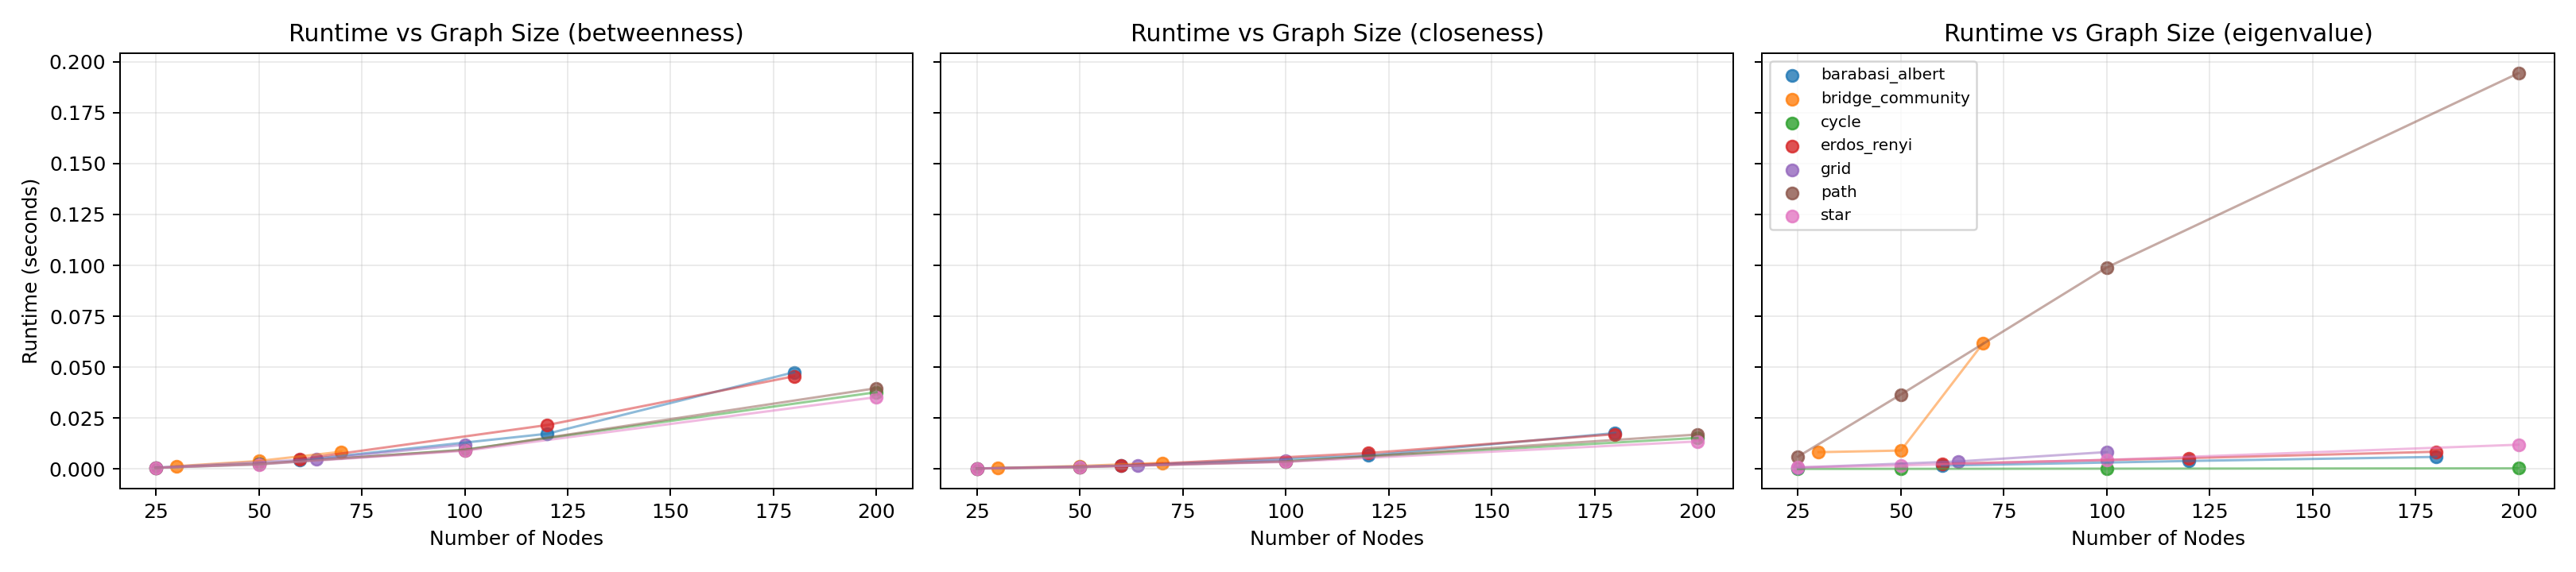
\includegraphics[width=0.9\textwidth]{figures/runtime_vs_graph_size.png}
\caption{Runtime scaling with graph size for each metric.}
\end{figure}

\begin{figure}[h!]
\centering
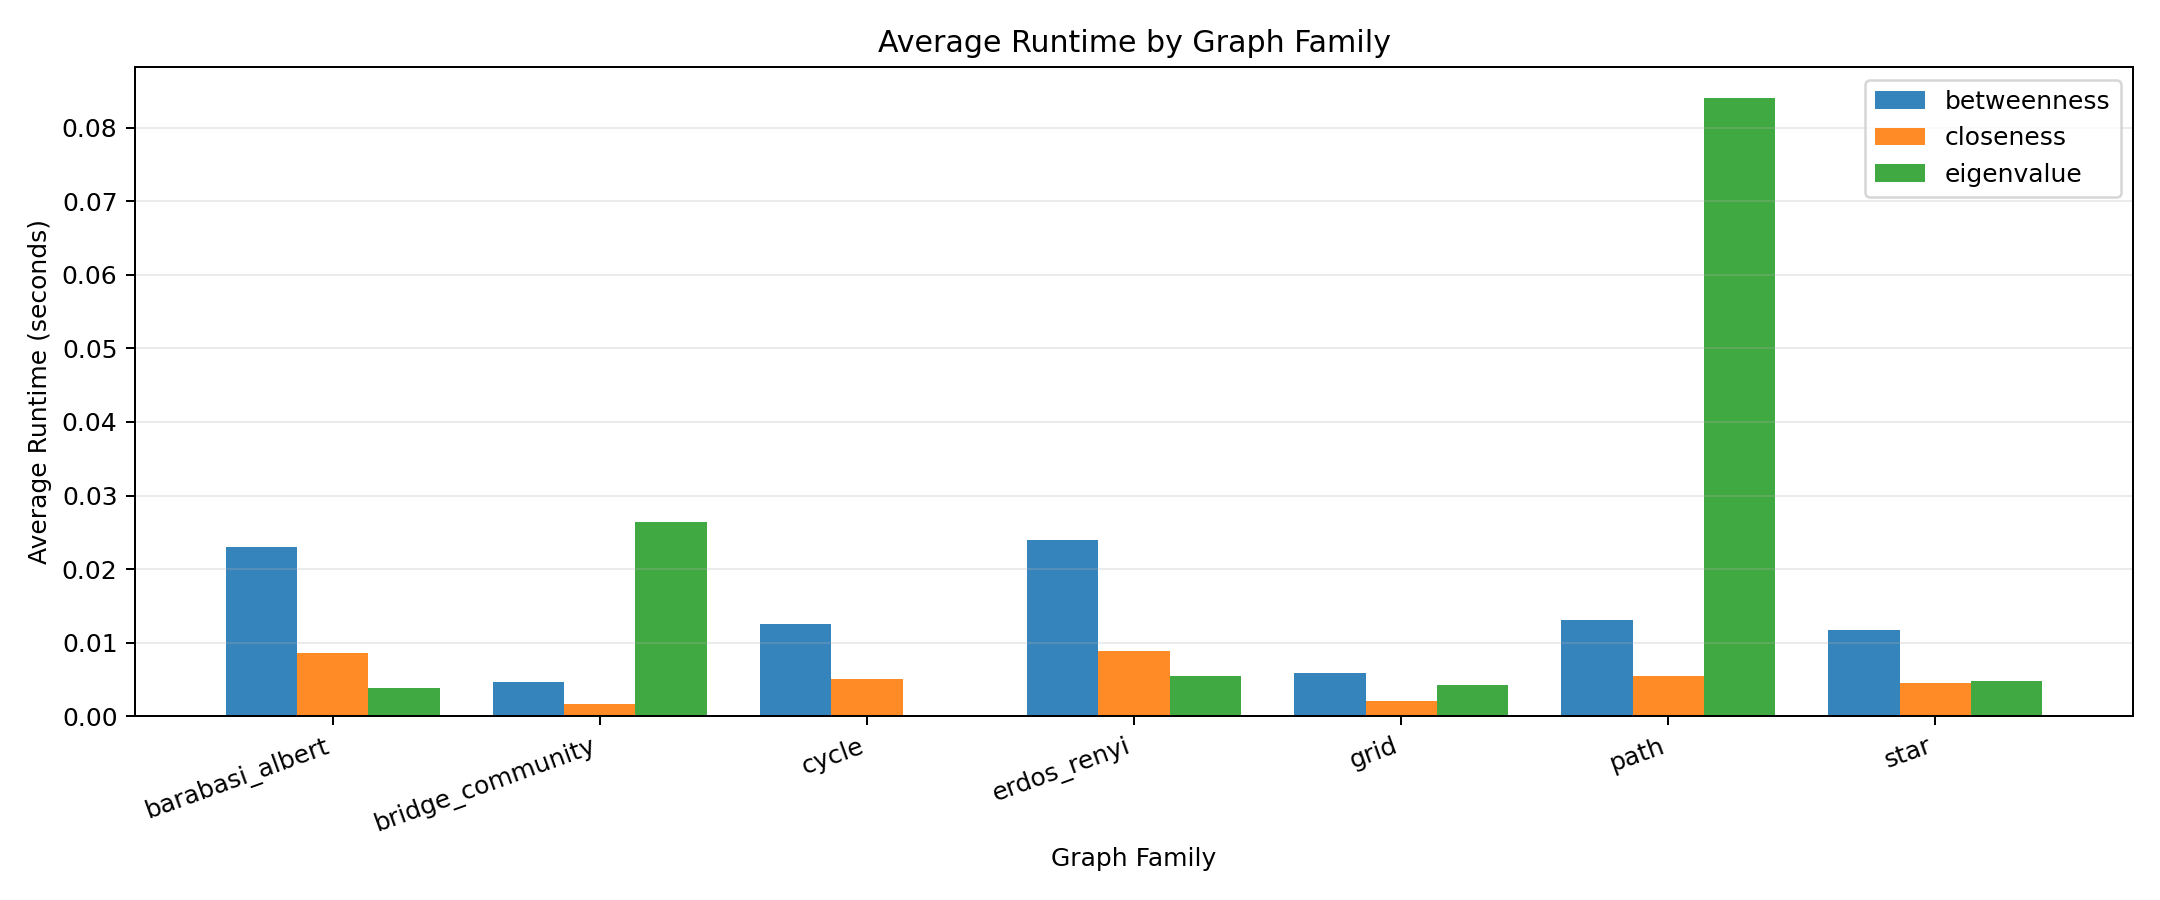
\includegraphics[width=0.9\textwidth]{figures/runtime_by_family.png}
\caption{Average runtime comparison across graph families.}
\end{figure}

The runtime plots show expected scaling trends: closeness and betweenness increase more sharply with graph size due to repeated BFS traversals, while eigenvalue runtime depends primarily on iteration count and graph sparsity.

\section{Comparative Analysis}
\begin{figure}[h!]
\centering
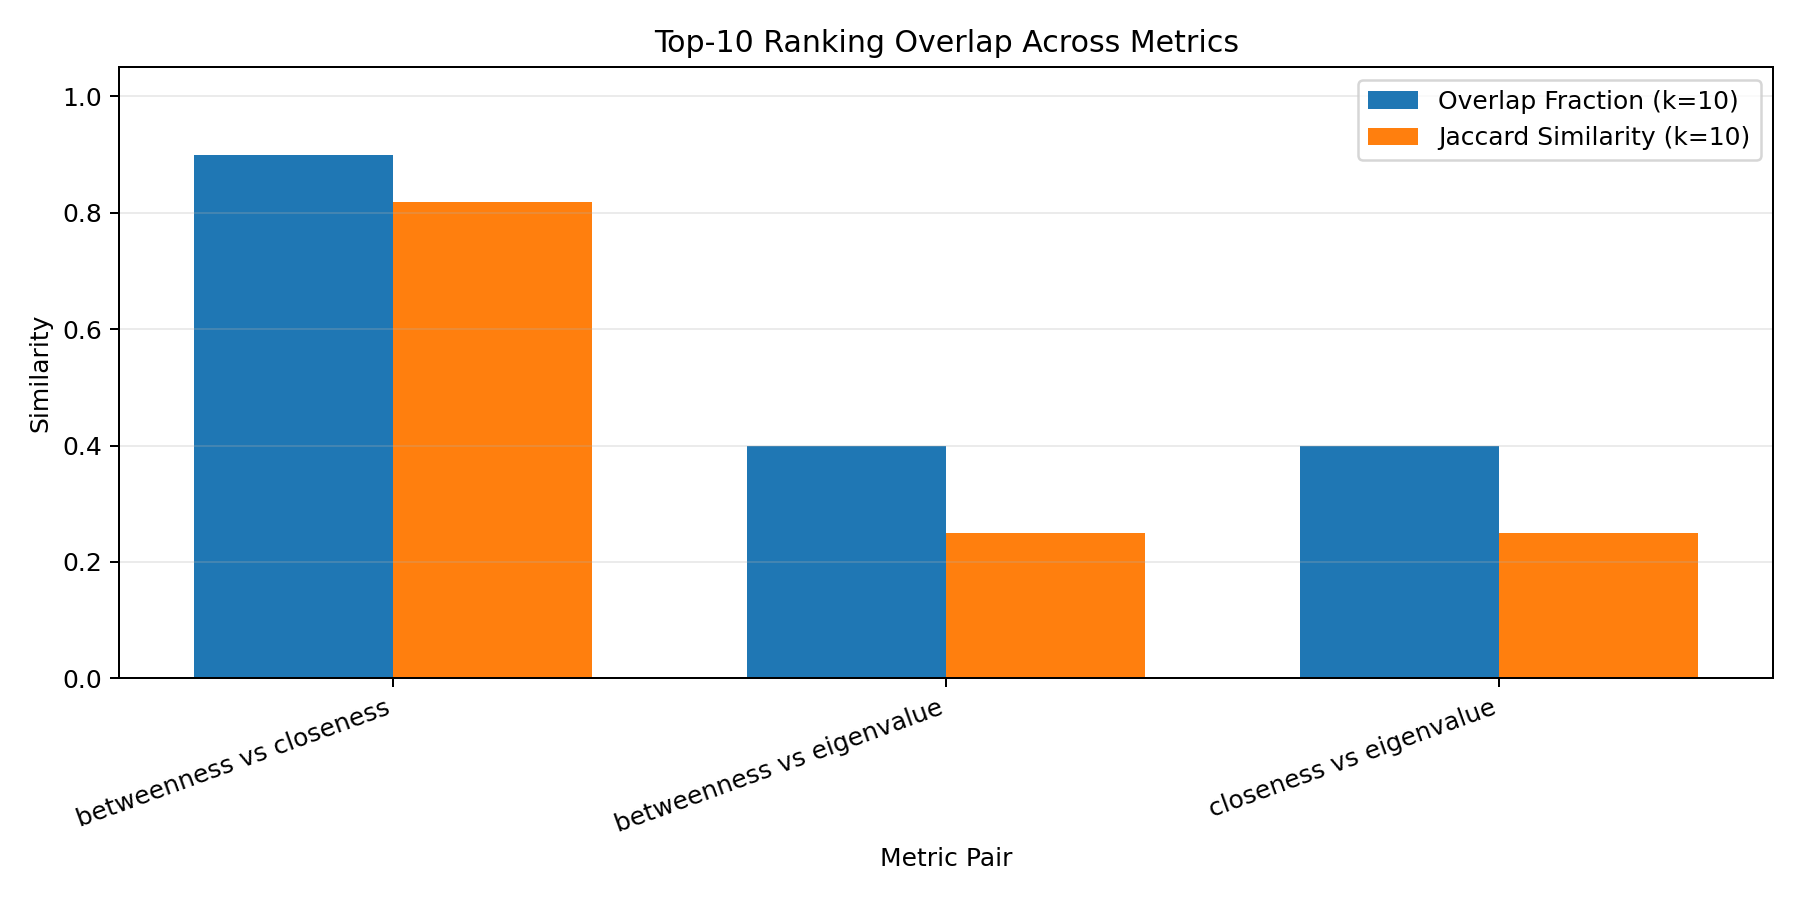
\includegraphics[width=0.9\textwidth]{figures/topk_overlap_bars.png}
\caption{Top-$k$ overlap and Jaccard similarity across metric pairs.}
\end{figure}

\begin{figure}[h!]
\centering
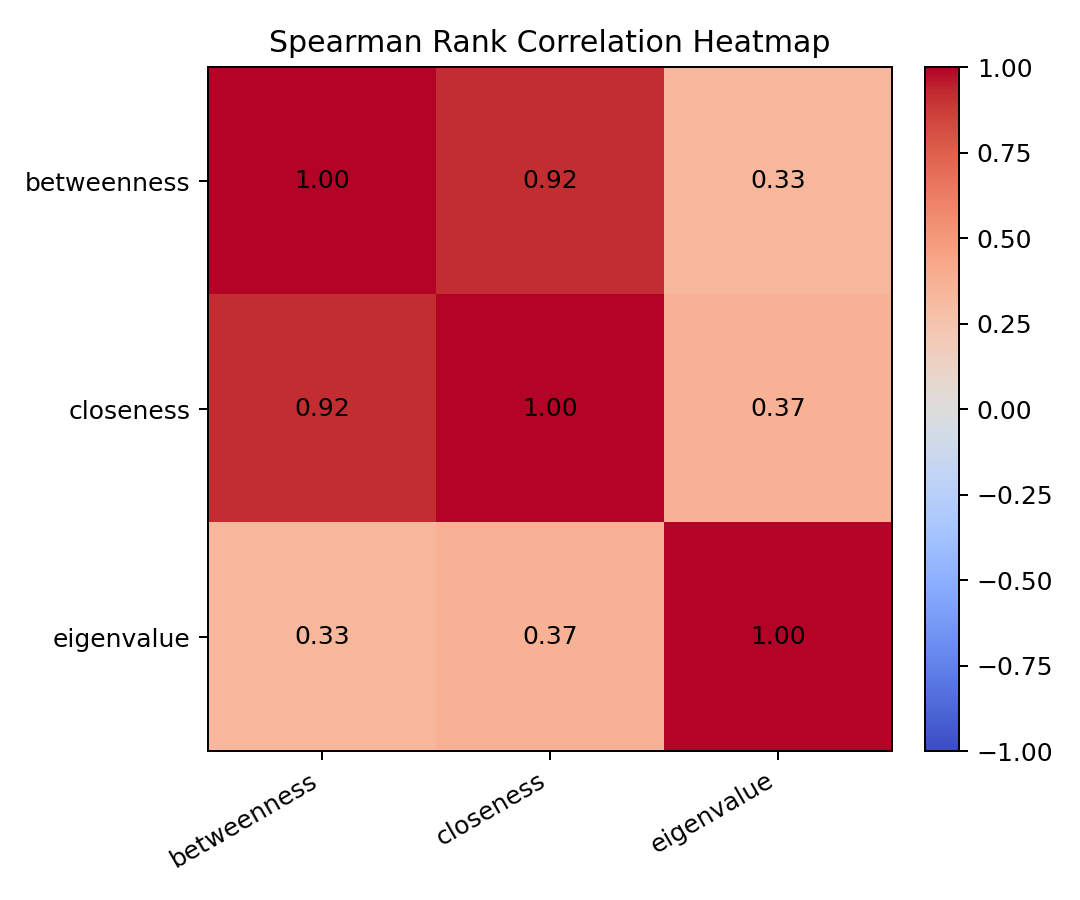
\includegraphics[width=0.8\textwidth]{figures/rank_correlation_heatmap.png}
\caption{Spearman rank correlation heatmap across centrality rankings.}
\end{figure}

\begin{figure}[h!]
\centering
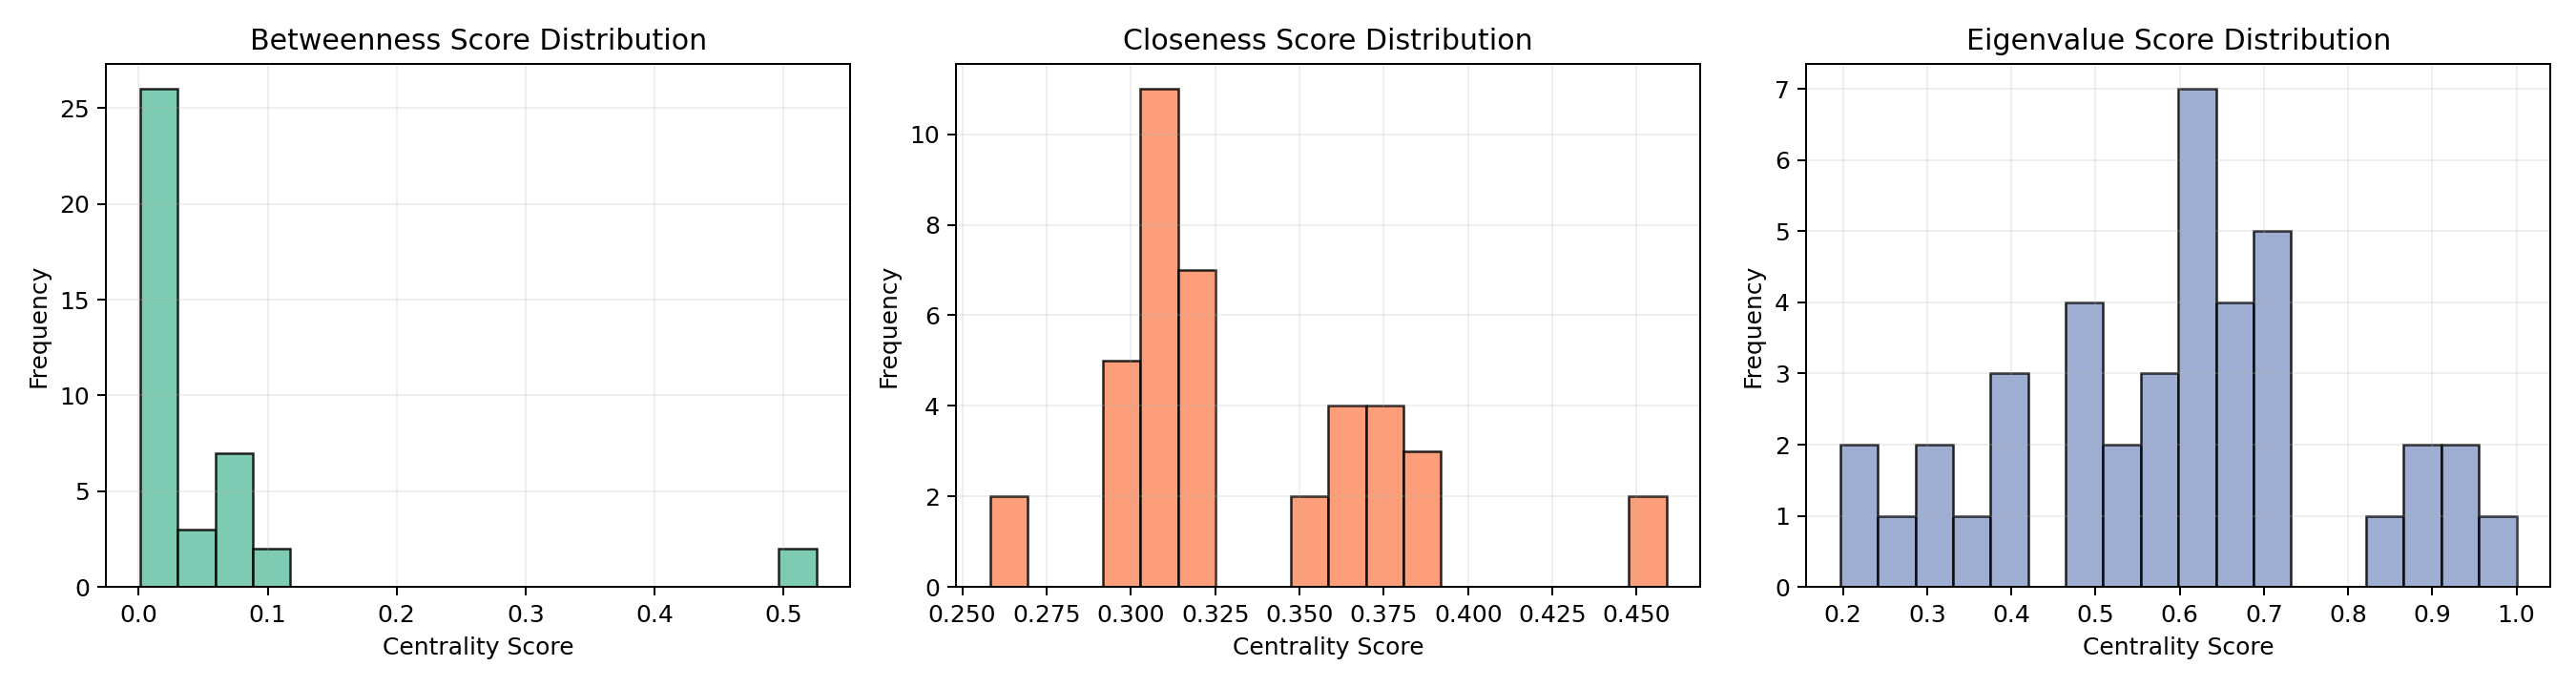
\includegraphics[width=0.9\textwidth]{figures/centrality_histograms.png}
\caption{Score distributions for implemented centrality metrics.}
\end{figure}

\section{Dashboard Description}
The Streamlit dashboard supports graph construction and upload, metric selection, summary inspection, graph rendering with centrality-driven encoding, ranking comparison, and CSV export of computed node scores.

\begin{figure}[h!]
\centering
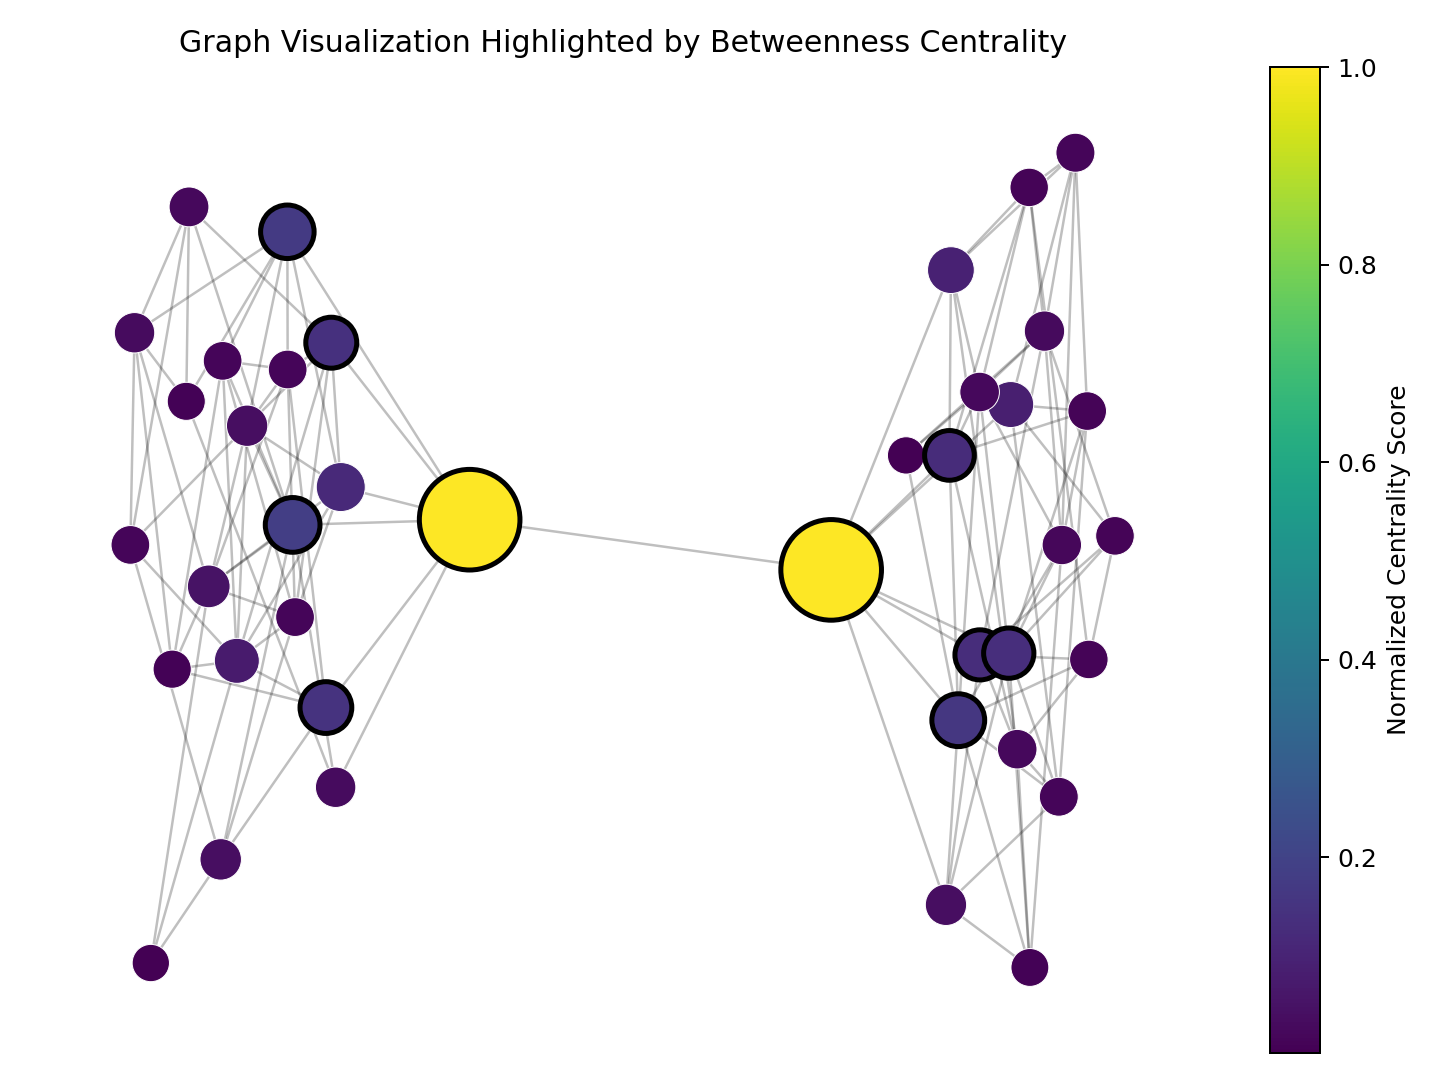
\includegraphics[width=0.85\textwidth]{figures/graph_highlight_betweenness.png}
\caption{Graph visualization highlighting high-betweenness nodes.}
\end{figure}

\section{Discussion}
The implemented metrics capture complementary notions of importance: closeness emphasizes global distance efficiency, betweenness captures brokerage on shortest paths, and eigenvalue rewards influence propagated through high-score neighborhoods. Comparative overlap and correlation reveal where these notions align and diverge on different graph structures.

\section{Limitations}
\begin{itemize}[leftmargin=*]
    \item Primary scope is unweighted undirected graphs.
    \item Benchmarking currently uses synthetic datasets only.
    \item Interactive dashboard is intended for small-to-medium graphs.
    \item Advanced statistical comparison methods beyond overlap and correlation are not included.
\end{itemize}

\section{Future Work}
\begin{itemize}[leftmargin=*]
    \item weighted and directed centrality variants,
    \item larger real-world datasets and ingestion pipelines,
    \item richer comparative statistics and stability analysis,
    \item enhanced interactive analytics and reporting features.
\end{itemize}

\section{Conclusion}
The project delivers a complete, modular centrality analysis platform with validated algorithm implementations, reproducible benchmarking, ranking comparison tooling, static visualization outputs, and an interactive dashboard. The resulting codebase provides a robust baseline for further comparative network analysis and applied graph analytics.

\end{document}
